\begin{figure}[ht]
  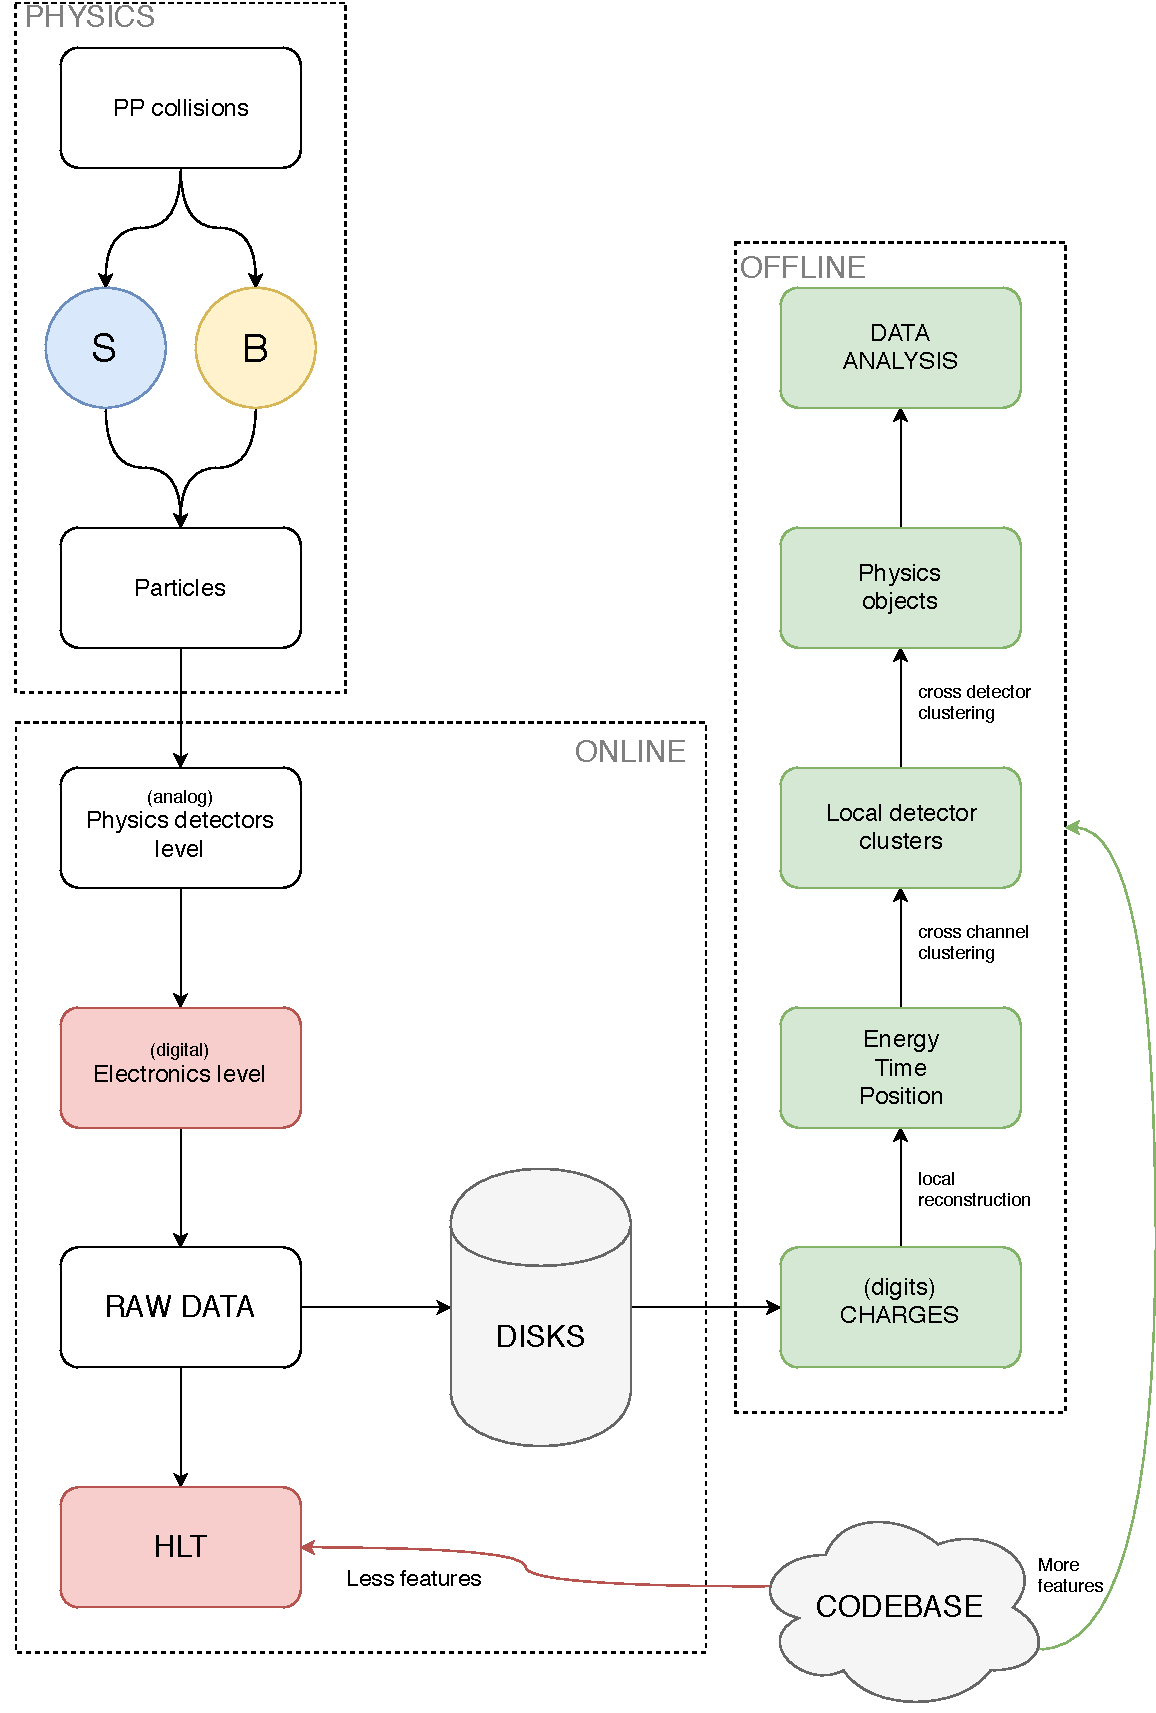
\includegraphics[height=\textheight]{img/dataflow}
  \caption{Cern data flow from collisions to analysis}
  \label{img:dataflow}
\end{figure}
% This might be an introduction
Modern high energy physics (HEP) requires analysis. To make it possible several large scale objects are needed: from accelerators, detectors, data centers to the thousands of people involved to design and run the infrastructure. Here at CERN everything starts with physics by colliding particles and everything ends with the physics performed by analyzing the data acquired. But, to produce the necessary data, in the right amount, a long and complicated process, showed in figure \ref{img:dataflow}, is involved. It is worth to briefly describe it to understand the reason of our work and where is it place inside it. \\
\paragraph{Data generation}
The process starts with \textbf{particle collisions} this lead to particle interactions that create some \textbf{intermediate product}. This intermediate product can not be directly observed, bit it decays in \textbf{particles} that go through the detectors. The intermediate product is divided in \textbf{X} and \textbf{Y}, X is what physicists are trying to study while Y is something that produces similar particles as Y but is not what they are looking for.
\paragraph{Data aquisition}
Detectors are split in two levels: \textbf{physics detector level} and \textbf{electronics level}. The physics level takes in input sensor readouts and produces an analog signal. This analog signal is the digitalized by the electronics level. This level also decides if the event is interesting or not, based on this the event is discarded or recorded. 
% Should I say that not interesting reading are discarded here?
The event that survive this ends up dumped into \textbf{disks} and send to the \textbf{High level trigger}. \\
It is important to notice that these decision are taken in real time, to meet the throughput and timing requirements everything is built with \textbf{asic}s and \textbf{fpga}s boards. 
\paragraph{Data processing} 
Data processing is performed both online and offline. %The \textbf{high level trigger} (HLT) performs it online while all the rest is offline. 
The first step, called \textbf{local reconstruction}, in the offline data processing is to transform charges in physical quantities such as \textbf{energy}, \textbf{time}, and \textbf{position}. This operation is done channel by channel independently form each other. Then, information coming from different channel of the same detector are combined by the \textbf{cross channel clustering} into \textbf{local detector cluster}s. The final step needed to obtain \textbf{particle object}s is the \textbf{cross detector clustering} in which data coming from different detector is combined. The particle object forms the dataset used by theoretical physicists to do physics. \\
\paragraph{High level trigger (HLT)}
The \textbf{HLT} belongs both to data acquisition and data processing, since it would not be correct to include it in one of this categories, it deserves a separate discussion. \\
The HLT main purpose is to select interesting events before writing them to disk. In order to accomplish this, it runs the same code used for the offline processing, but \textbf{online} and with less features because of strict time constraints. \\
The main difference between \textbf{L1} and HLT is that L1 is implemented in hardware with no host while HLT is software based, it runs on hosts with accelerators used to speed-up the processing.